\documentclass[12pt]{article}
%\documentclass{article}

\usepackage{times}
\usepackage[final]{graphicx}
\usepackage{hyperref}
\usepackage{verbatim}
\usepackage{color}
\usepackage{amsmath}
\setlength{\topmargin}{-0.5in}
\setlength{\oddsidemargin}{0in}
\setlength{\evensidemargin}{0in}
\setlength{\textwidth}{6.5in}
\setlength{\textheight}{9.0in}

\begin{document}

\centerline{\bf \Large CS295/CS395/CSYS395: \href{CS295_395_Syllabus.pdf}{\underline{Evolutionary Robotics}}}

\vspace{0.5cm}

\centerline{\bf \large Programming Assignment 5b of 10}
\vspace{0.25cm} \centerline{\color{red}DRAFT: Port from ODE to Bullet by Shane Celis \color{black}}

\vspace{0.5cm}

\centerline{\large Assigned: Friday, September 30, 2011}

\vspace{0.5cm}

\centerline{\large Due: Friday, October 7, 2011 by midnight}

\vspace{0.5cm}

\noindent \color{red}CHANGES: The coordinate reference frame is slightly different than ODE.\color{black}\\

\noindent \textbf{Description:} In this assignment you will start with the `empty' simulation you created in assignment 4 and incrementally add objects to construct a quadrupedal robot. In the next assignment you will add joints to your simulation so that the objects are connected together, then sensors, then motors, and then a controlling neural network.

\begin{enumerate}

\item Create a directory, Assignment\_4, that contains your assignment 4 submitted document. Copy the bullet-2.79 directory into this directory as well. Back up this directory. Now in subsequent assignments if you find your simulation becomes unusable you can go back and retrieve the `empty' simulation stored in this directory.

\item Create a new directory, Assignment\_5, and copy the bullet-2.79 directory here. For the remainder of this assignment make changes to the files in this ode directory.

\item Draw the image shown in Fig. \ref{Fig1} on a blank sheet of paper. Draw to fill an entire page, as you will be annotating the image through the next few assignments.

\begin{figure}[!t]
\centerline{
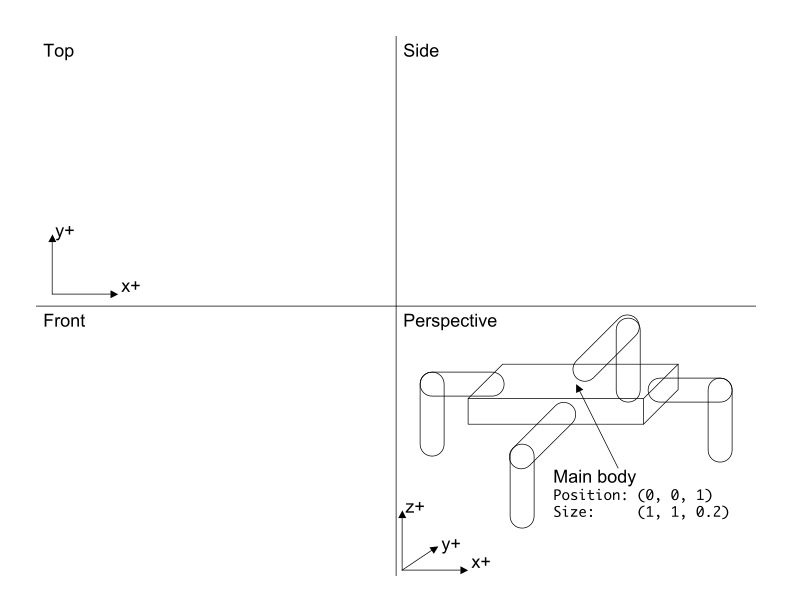
\includegraphics[width=1.0\textwidth]{Robot_Schematic}
}
\caption{A template for sketching the quadrupedal robot to be simulated.}
\label{Fig1}
\end{figure}

\item Now draw the robot from the three additional perspectives as we did in class.

\item For the four upper and four lower legs, mark their positions, sizes (radius and length) and orientations (see Lecture 6, slide 4) in the three panels. You can choose the lengths and radii of the legs to your liking.

\item Now, in the \texttt{RagdollDemo.h} program, we need to create
  body and geom data structures to store all the objects that make up
  the robot. Find the member variable declarations for the RagdollDemo class

\begin{verbatim}
class RagdollDemo : public GlutDemoApplication
{
  btAlignedObjectArray<class RagDoll*> m_ragdolls;
  //keep the collision shapes, for deletion/cleanup
  btAlignedObjectArray<btCollisionShape*> m_collisionShapes;
  btBroadphaseInterface*  m_broadphase;
  btCollisionDispatcher*  m_dispatcher;
  btConstraintSolver* m_solver;
  btDefaultCollisionConfiguration* m_collisionConfiguration;
  btDefaultCollisionConfiguration* m_collisionConfiguration;
\end{verbatim}

and add the following variables:

\begin{verbatim}
    btRigidBody*      body[9]; // one main body, 4x2 leg segments
    btCollisionShape* geom[9];
    bool pause;
\end{verbatim}

\item Recompile the code. If you get errors, delete those parts of the code that refer to the variables you deleted. Continue this process until you compile and run without errors.

\item Now you will create some functions that can be used to add objects to the empty simulator. Create a function of the form \\
\texttt{void CreateBox( int index,}\\
\texttt{        double x, double y, double z,}\\
\texttt{        double length, double width, double height) \{}\\
\texttt{  ...}\\
\texttt{  body[index] = ...}\\
\texttt{  ...}\\
\texttt{  geom[index] = ...}\\
\texttt{  ...}\\
\texttt{\}} \\
which will be used to create the main body of the robot. Refer to the commented-out code to figure out how to create an object. Assume the mass of all objects for now is 1. Without calling the function, recompile and run until you have no errors.

\item Create a similar function for creating cylinders \verb|CreateCylinder(index,...)|, which will be used to create the upper and lower legs of the robot. You will need to add additional parameters for specifying the orientation of the cylinder. Recompile and run until error-free.

\item Create another function \\
\texttt{void DeleteObject( int index ) \{}\\
\texttt{  ...}\\
\texttt{\}} \\
which can be used to remove objects from the simulation. This function should destroy both the body and the geom associated with the object using \texttt{delete}. Recompile and run until error-free.

\item Now, in the \verb|initPhysics| method in \verb|RagdollDemo.cpp|, add code to create the first object

\begin{verbatim}
  //spawnRagdoll(startOffset);  Commented out in exercise 4b.
  CreateBox(0, 0., 1., 0., 1., 0.2, 1.); // Create the box
  clientResetScene();   
\end{verbatim}
Compile and run until error-free.  You should see the box fall and come to rest on the ground as in Fig. \ref{Fig2}a. (You can toggle texture drawing by hitting the 'u' key.) Screencapture this image and paste into your document.

\item Create box will allocate memory for the body and geom objects.  As it is, our simulation will run, but it will leak memory.  If you reset the simulation enough times by hitting the space bar, it will eventually run out of memory.  So we need to delete the objects.  In \verb|RagdollDemo|'s deconstructor method \small{$\sim$}\verb|RagdollDemo| delete the object. 
\begin{verbatim}
  virtual ~RagdollDemo()
  {
    DeleteObject(0);
    exitPhysics();
  }
\end{verbatim}

\item We're going to add the ability to pause the simulation.  Modify the call to \verb|stepSimulation| to look like the following.

\begin{verbatim}
  if (!pause) {
    m_dynamicsWorld->stepSimulation(ms / 1000000.f);
  }
\end{verbatim}
Recompile until there are no errors.  Note that the simulation can technically be paused, but there's currently no means of pausing it from the UI.  

\item We want to be able to toggle whether the simulation is paused while it is running.  Modify the method \verb|keyboardCallback| in \verb|RagdollDemo.cpp| to toggle the variable \verb|pause| when the key 'p' is pressed.  Recompile and run and verify that after 'p' is pressed, the simulation is paused.  When 'p' is pressed again, the simulation continues running.  

\item Now pause your simulation by hitting 'p', then reset your simulation by hitting the space key.  You should see the box hanging in midair as in Fig. \ref{Fig2}b. Screencapture and paste into your document. Hitting 'p' will unpause the simulation and cause the object to fall to the ground.

\item Add \texttt{CreateCylinder(1,...)} after the call to \verb|CreateBox(0,...)| is called to add the next object to the robot. Note that you will have to specify the orientation of the cylinder, which you do not have to do for the main body. When run in paused mode you should see both objects as in Fig. \ref{Fig2}c. Screencapture and copy and paste into your document.

\item Add a third object, compile, run and ensure that the object appears where you expect it. Continue to add an object and recompile until all nine objects are added. This should produce a simulation as shown in Fig. \ref{Fig2}d. Screencapture, copy and paste into your document, and submit.
\end{enumerate}

\begin{figure}[!t]
\centerline{
a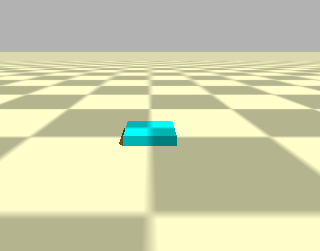
\includegraphics[width=0.4\textwidth]{fig2a}
b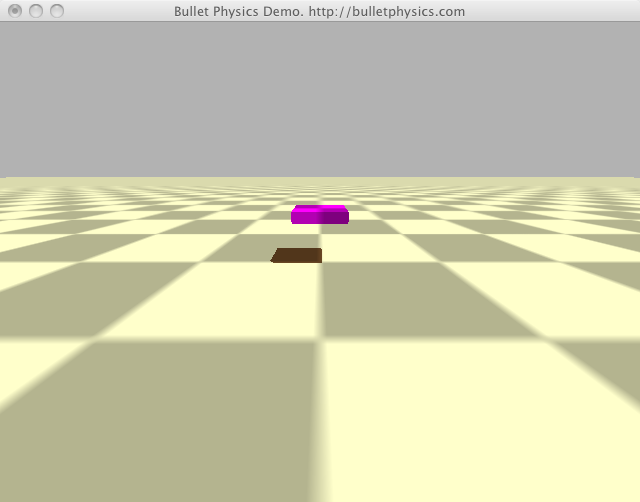
\includegraphics[width=0.4\textwidth]{fig2b}
}
\centerline{
c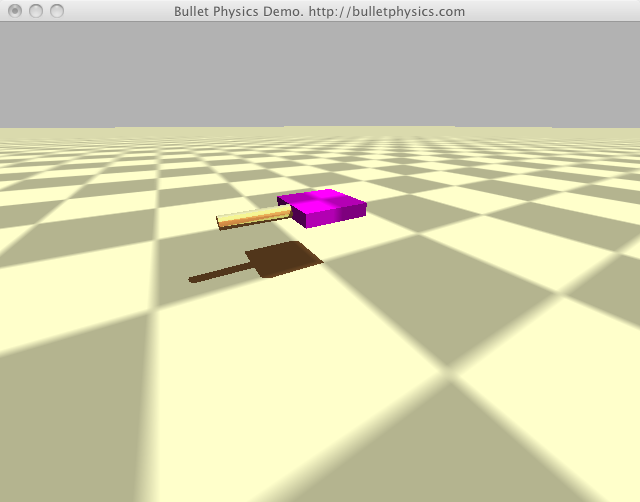
\includegraphics[width=0.4\textwidth]{fig2c}
d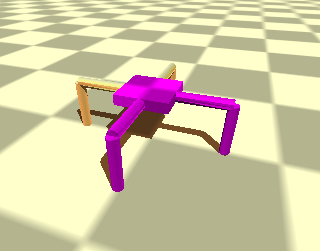
\includegraphics[width=0.4\textwidth]{fig2d}
}
\caption{The quadrupedal robot under construction in ODE.}
\label{Fig2}
\end{figure}

\end{document} 
